% Document setup
\documentclass[12pt]{article}
\usepackage[margin=1in]{geometry}
\usepackage{fancyhdr}
\usepackage{lastpage}

\pagestyle{fancy}
\lhead{Richard Whitehill}
\chead{PHYS 804 -- HW \HWnum}
\rhead{\duedate}
\cfoot{\thepage \hspace{1pt} of \pageref{LastPage}}

% Encoding
\usepackage[utf8]{inputenc}
\usepackage[T1]{fontenc}

% Math/Physics Packages
\usepackage{amsmath}
\usepackage{amssymb}
\usepackage{mathtools}
\usepackage{physics}
\usepackage{siunitx}

\AtBeginDocument{\RenewCommandCopy\qty\SI}

% Enumeration/itemize
\usepackage{enumitem}
\newenvironment{parts}
{\begin{enumerate}[label=\textbf{(\alph*)},leftmargin=*,itemsep=-10pt]
}{\end{enumerate}}

% Reference Style
\usepackage{hyperref}
\hypersetup{
    colorlinks=true,
    linkcolor=blue,
    filecolor=magenta,
    urlcolor=cyan,
    citecolor=green
}

\newcommand{\eref}[1]{Eq.~(\ref{eq:#1})}
\newcommand{\erefs}[2]{Eqs.~(\ref{eq:#1})--(\ref{eq:#2})}

\newcommand{\fref}[1]{Fig.~\ref{fig:#1}}
\newcommand{\frefs}[2]{Figs.~\ref{fig:#1}--\ref{fig:#2}}

\newcommand{\tref}[1]{Table~\ref{tab:#1}}
\newcommand{\trefs}[2]{Tables~\ref{tab:#1}-\ref{tab:#2}}

% Figures and Tables 
\usepackage{graphicx}
\usepackage{float}
\usepackage[font=small,labelfont=bf]{caption}

\newcommand{\bef}{\begin{figure}[h!]\begin{center}}
\newcommand{\eef}{\end{center}\end{figure}}

\newcommand{\bet}{\begin{table}[h!]\begin{center}}
\newcommand{\eet}{\end{center}\end{table}}

% tikz
\usepackage{tikz}
\usetikzlibrary{calc}
\usetikzlibrary{decorations.pathmorphing}
\usetikzlibrary{decorations.markings}
\usetikzlibrary{arrows.meta}
\usetikzlibrary{positioning}
\usetikzlibrary{3d}
\usetikzlibrary{shapes.geometric}

% tcolorbox
\usepackage[most]{tcolorbox}
\usepackage{xcolor}
\usepackage{xifthen}
\usepackage{parskip}

\newcommand*{\eqbox}{\tcboxmath[
    enhanced,
    colback=black!10!white,
    colframe=black,
    sharp corners,
    size=fbox,
    boxsep=8pt,
    boxrule=1pt
]}

% problem-solution macros
% \usepackage{adjustbox}
\usepackage{changepage}

\newtcolorbox{probbox}[1][]{
    breakable,
    enhanced,
    boxrule=0pt,
    frame hidden,
    borderline west={4pt}{0pt}{green!50!black},
    colback=green!5,
    before upper=\textbf{Problem #1) \,},
    % \textbf{Problem #1 \ifthenelse{\isempty{#1}}{}{: #1} \\ },
    sharp corners,
    parbox=false
}

% \newtcolorbox{ProblemBox}[1][]{%
%   breakable,
%   enhanced,
%   colback=black!10!white,
%   colframe=black,
%   title={\large #1 \hfill}
% }
\newcommand{\prob}[2]{
\begin{probbox}[#1]
#2
\end{probbox}
}

\newenvironment{solution}{\begin{adjustwidth}{8pt}{8pt}}{\end{adjustwidth}}
\newcommand{\sol}[1]{
\begin{solution}
#1
\end{solution}
}
% \textbf{#1)} #2}

% Miscellaneous Definitions/Settings
\newcommand{\reals}{\mathbb{R}}
\newcommand{\integers}{\mathbb{Z}}
\newcommand{\naturals}{\mathbb{N}}
\newcommand{\rationals}{\mathbb{Q}}
\newcommand{\complexs}{\mathbb{C}}

\setlength{\parskip}{\baselineskip}
\setlength{\parindent}{0pt}
\setlength{\headheight}{14.49998pt}
\addtolength{\topmargin}{-2.49998pt}


\def\HWnum{Project 3}
\def\duedate{November 10, 2024}


\begin{document}

\section{Introduction}
\label{sec:introduction}

In this project, we will be interested in finding bound states of a quantum system.
This requires us to solve the time-independent Schr\"{o}dinger equation or energy eigenvalue equation
\begin{align}
    -\frac{\hbar^2}{2m} \dv[2]{\psi(x)}{x} + V(x) \psi(x) = E \psi(x)
,\end{align}
where $\psi(x)$ is the wave-function of our system, $V(x)$ is the potential, and $E$ is an energy eigenvalue.
Note that for simplicity we work in one-dimension.
Such a problem is of great importance in physics given that the Schr\"{o}dinger equation is the fundamental equation which governs the behavior and characteristics of a system.

This article is organized as follows.
In Sec. \ref{sec:theoretical-framework-and-numerical-implementation}, we outline the theoretical underpinnings to cast the problem in a manner compatible with a computer program and discuss the numerical methods used to solve the energy eigenvalue equation numerically.
Next, in Sec. \ref{sec:results}, we apply the developed code to a myriad of example potentials $V(x)$ and discuss some observations.
Finally, in Sec. \ref{sec:conclusion}, we summarize our findings and briefly discuss some possible improvements to the numerical implementation and interesting future explorations.


\section{Theoretical framework and numerical implementation}
\label{sec:theoretical-framework-and-numerical-implementation}

The energy eigenvalue equation above is a second-order ordinary differential equation, where $E$ is not specified.
Formally, this is a Sturm-Liouville problem, which is a subject of great interest in both the fields of mathematics and physics.
For our purposes here, we would first like to cast this equation in a system of convenient units or make the relevant quantities dimensionless.
First, observe that we can write
\begin{align}
    -\dv[2]{\tilde{\psi}}{x} + \frac{2 m V(x)}{\hbar^2} \tilde{\psi} = \frac{2 m E}{\hbar^2} \tilde{\psi}
.\end{align}
Next, for most problems, we can find a relevant length scale $a$, allowing us to define a dimensionless parameter $u = x/a$.
Doing so, our equation becomes
\begin{align}
\label{eq:dimless-SE}
    -\dv[2]{\psi}{u} + v(x) \psi = \varepsilon \psi
,\end{align}
where we have defined $v(x) = 2 m a^2 V(x) / \hbar^2$ and $\varepsilon = 2 m a^2 E / \hbar^2$ as well as $\tilde{\psi}(x) = \sqrt{a} \psi(x)$.
The latter choice has been made since the norm-squared of the wave-function is a probability density, which must obey
\begin{align}
    \int \dd{x} |\psi(x)|^2 = \int \dd{u} |\tilde{\psi}(u)|^2 = 1
,\end{align}
and hence, $\tilde{\psi}$ is dimensionless.
This is all the massaging we will perform before introducing our numerical methods.

There are several treatments one can use to broach solving Eq. (\ref{eq:dimless-SE}).
Here, we will transform the continuous differential equation into a matrix equation.
We first choose an interval $[a,b]$ on which to solve the equation and impose Dirichlet boundary conditions with $\psi(a) = \psi(b) = 0$.
Next, we set up a lattice of $N + 2$ points $x_{n} = x_0 + n h$, where $h = (b - a)/(N+1)$ such that $x_0 = a$ and $x_{N=1} = b$.
Because we no longer have a continuous domain, we instead approximate the derivative using the central difference formula from the finite difference method:
\begin{align}
    \tilde{\psi}''(x_{n}) = \frac{\tilde{\psi}(x_{n-1}) - 2 \tilde{\psi}(x_{n}) + \tilde{\psi}(x_{n+1})}{h^2}
.\end{align}
Because of the discretization, we have we have $N$ equations for the interior points of our interval:
\begin{align}
\begin{aligned}
    -\frac{1}{h^2} \Big[ -2 \tilde{\psi}(x_1) + \tilde{\psi}(x_2) \Big] + V(x_{1}) \psi(x_1) &= E \psi(x_1) \\
    -\frac{1}{h^2} \Big[ \tilde{\psi}(x_1) - 2 \tilde{\psi}(x_2) + \tilde{\psi}(x_3) \Big] + V(x_{1}) \psi(x_2) &= E \psi(x_2) \\
    \vdots \\
    -\frac{1}{h^2} \Big[ \tilde{\psi}(x_{N-2}) - 2 \tilde{\psi}(x_{N-1}) + \tilde{\psi}(x_{N}) \Big] + V(x_{1}) \psi(x_{N-1}) &= E \psi(x_{N-1}) \\
    -\frac{1}{h^2} \Big[ \tilde{\psi}(x_{N-1}) - 2 \tilde{\psi}(x_{N}) \Big] + V(x_{1}) \psi(x_{N}) &= E \psi(x_{N})
.\end{aligned}
\end{align}
If we form the wave-function vector $\tilde{\psi} = \begin{pmatrix} \tilde{\psi}(x_{1}) \hdots \tilde{\psi}(x_{N}) \end{pmatrix}^{\rm T}$, we have an equation of the form $H \tilde{\psi} = E \tilde{\psi}$, where our discretized Hamiltonian matrix elements
\begin{align}
    H_{nm} = -\frac{1}{h^2} \delta_{n,m-1} + \Big[ \frac{2}{h^2} + V(x_{n}) \Big] \delta_{nm} - \frac{1}{h^2} \delta_{n,m+1}
.\end{align}
Once this matrix is set up, we use the eigensolver \textit{scipy.linalg.eigh\_tridiagonal} to find the spectrum of our system, making use of the fact that our matrix is tridiagonal and saving only the solutions corresponding to bound states of our potential.


\section{Results}
\label{sec:results}

\subsection{Finite square well}
\label{ssec:finite-square-well}

For our first potential, we analyze the finite square well with
\begin{align}
    V(x) = \begin{cases}
        0 & |x| < a \\
        V_0 & {\rm otherwise}
    .\end{cases}
\end{align}
This is a useful potential for stress-testing our code given that we can solve for the functional form of the wave-function exactly
\begin{align}
    \tilde{\psi}(x) = \begin{cases}
        A e^{\kappa u} & u < -1 \\
        B \cos{k u} + C \sin{k u} & |u| < 1 \\
        D e^{-\kappa u} & u > 1
    ,\end{cases}
\end{align}
where $k^2 = \varepsilon$ and $\kappa^2 = \sqrt{v_0 - \varepsilon}$ with $v_0 = 2 m a^2 V_0 / \hbar^2$.
Applying the relevant boundary conditions, we find even and odd solutions with either $C = 0$ or $B = 0$ and energies which satisfy the transcendental equations
\begin{align}
\label{eq:finite-well-energy-cond}
    \pm k \tan{k} = \kappa
,\end{align}
with the $+$ and $-$ branches corresponding to even and odd solutions, respectively.
An example of these solutions is shown in Fig. \ref{fig:finite-well-exact-solutions} with $v_0 = 100$.
With these solutions for the energies in hand, we can normalize our wave-function and determine all the constants $A,\,B,\,C,\,{\rm and}\,D$.

\begin{figure}[h!tb]
    \centering
    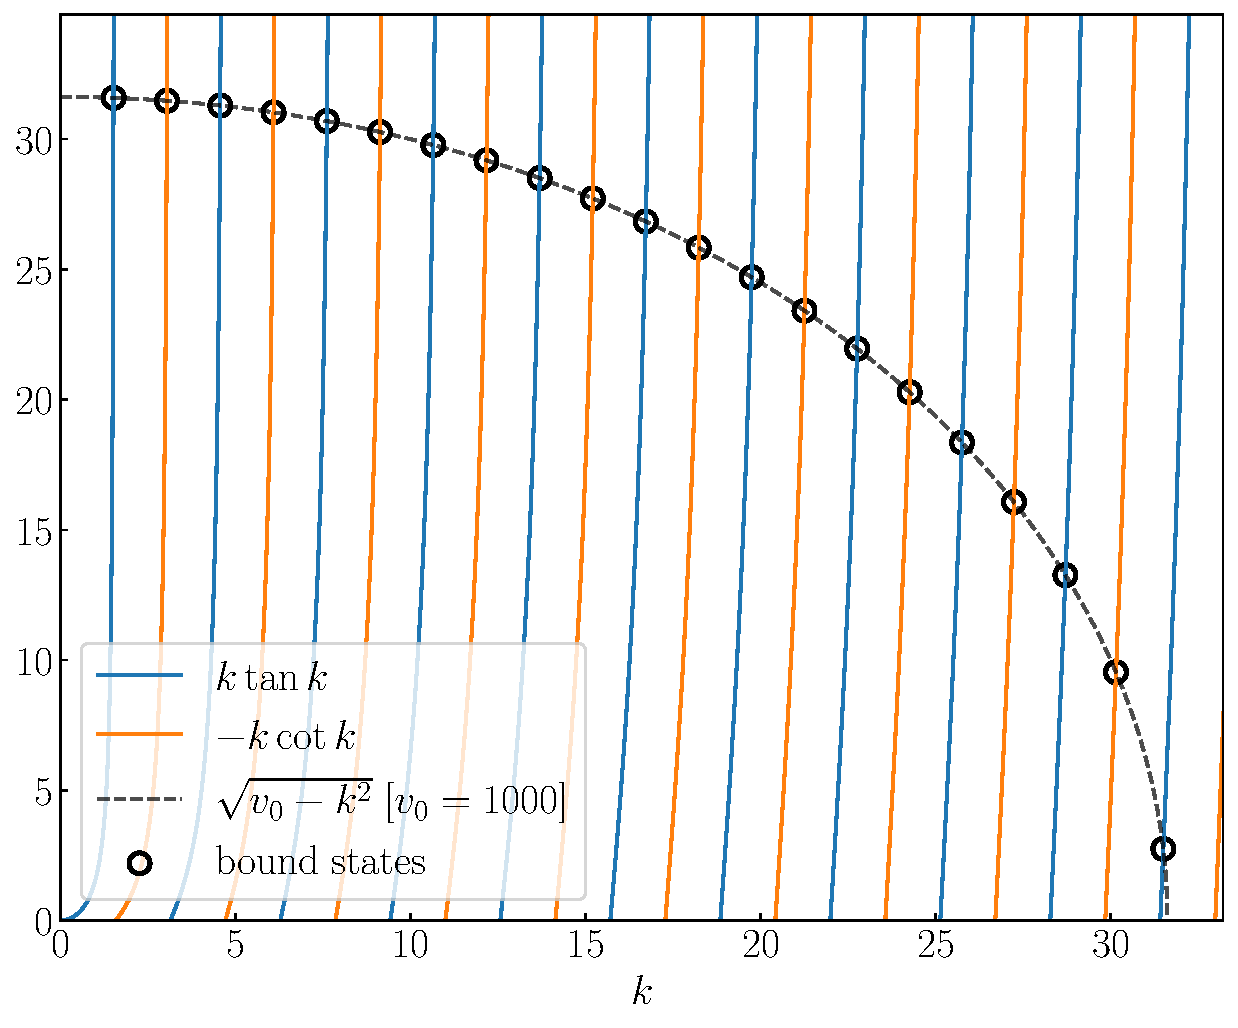
\includegraphics[width=0.5\linewidth]{finite_well_exact_solutions.pdf}
    \caption{Curves for the left and right hand side of Eq. (\ref{eq:finite-well-energy-cond}) for even and odd cases with $v_0 = 100$. The open, black circles correspond to solutions of the transcendental equation and therefore bound state energies.}
    \label{fig:finite-well-exact-solutions}
\end{figure}

In Fig. \ref{fig:finite-well-wfs}, we compare the numerical solutions for the wave-function and analytic results for a selection of interval widths, increasing from top to bottom, and lattice points, increasing from left to right.
One can see in the upper-left panel that the numerical result follows the analytic one fairly well until it reaches the artificial boundary because we impose Diricihlet boundary conditions but do not have a wide enough interval for the wave-function to approach close enough to zero.
In the upper-right panel, we have a similar issue, where the analytic solution is reproduced quite well in the well but begins to deviate a bit once outside.
Next, in the lower-left panel, we have a different issue.
Now, we have allowed our interval to be wide enough to accurately reproduce the asymptotic behavior with our Dirichlet boundary conditions, but we do not have enough lattice points to accurately construct the behavior of the wave-function near the well.
To amend this behavior, in the lower-right panel, we increase the number of lattice points and find good agreement between the numerical and analytic results.

\begin{figure}[h!tb]
    \centering
    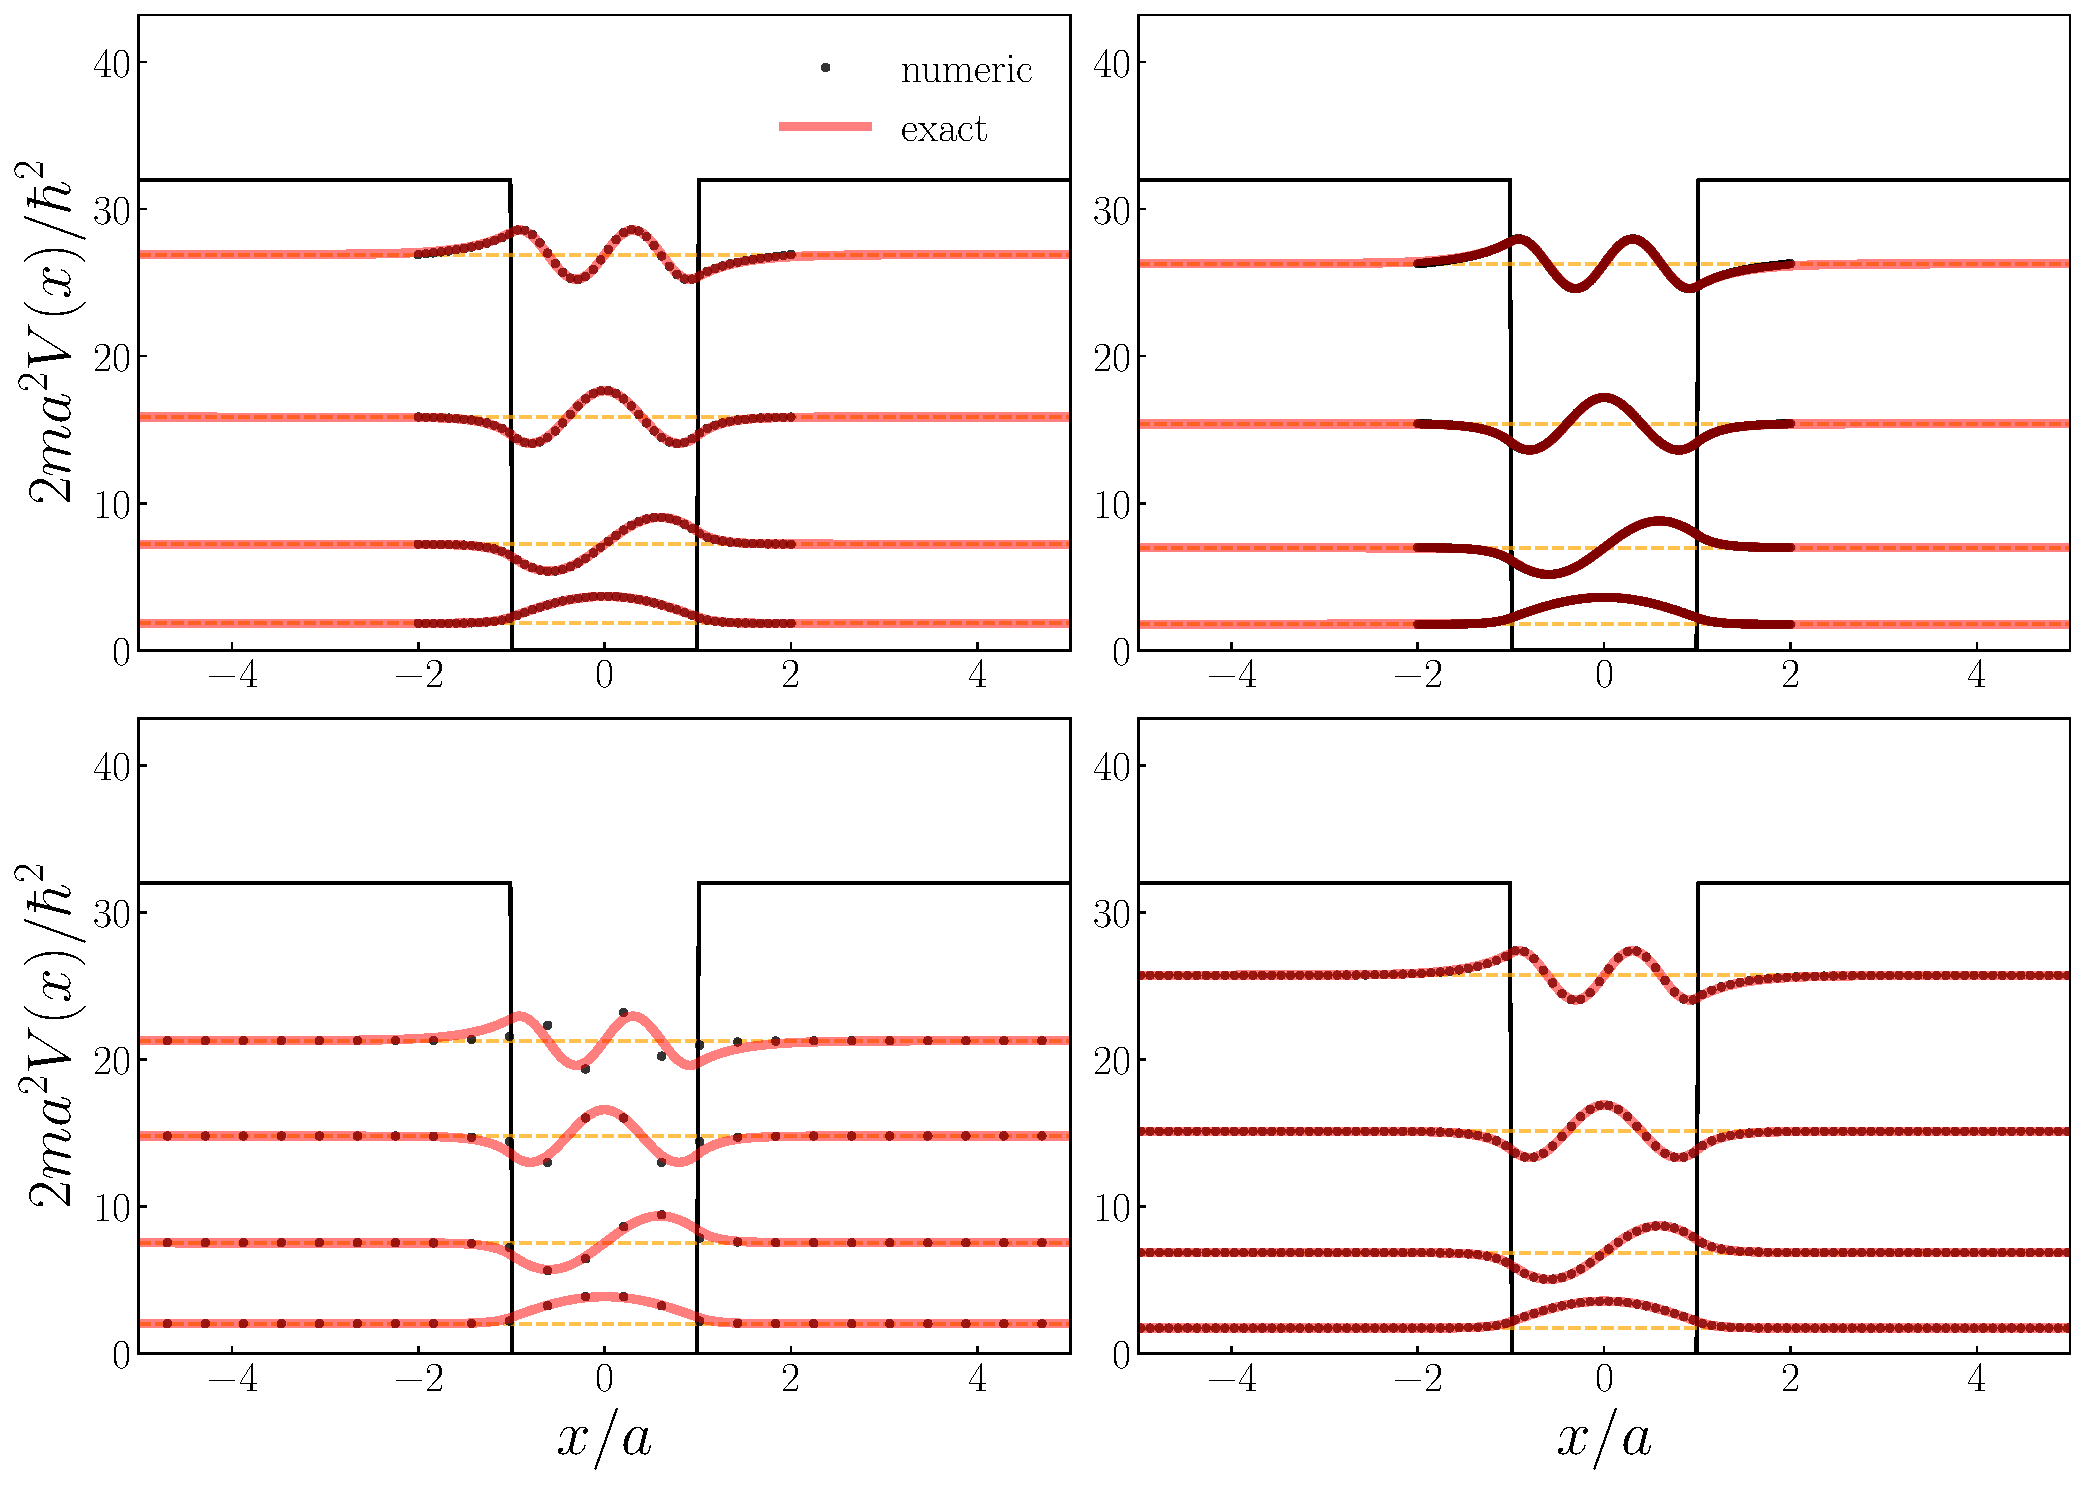
\includegraphics[width=\linewidth]{finite_well_wfs.pdf}
    \caption{Plot of the numerical and analytic results for the first four wave-functions of the finite potential well for a selection of interval widths (top row: $[-2,2]$, bottom row: $[-10,10]$) and lattice points (left column: $N = 50$, right column: $N = 200$).}
    \label{fig:finite-well-wfs}
\end{figure}

As a final test, we observe that in the limit $V_0 \rightarrow \infty$, we obtain the infinite square well, which has an exactly known energy spectrum
\begin{align}
    \varepsilon_{n} = \frac{\pi^2}{4} n^2
.\end{align}
In Fig. \ref{fig:finite-well-spectrum}, we plot the ratio of the first-four energy eigenvalues to the first and divide by $n^2$ for a selection of $v_0$.
We can see that as we increase $v_0$, the eigenvalues approach the exact ones, although across the board, we have accuracy $\lesssim 1\%$.

\begin{figure}[h!tb]
    \centering
    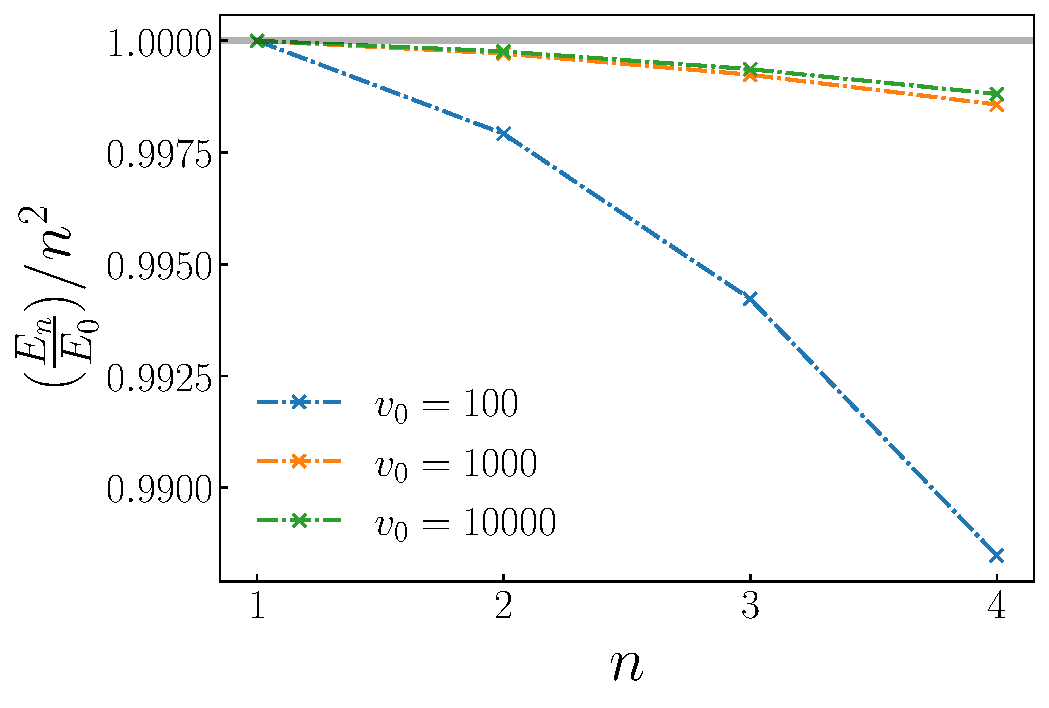
\includegraphics[width=0.5\linewidth]{finite_well_spectrum.pdf}
    \caption{Ratio of reduced energies $E_{n}/E_0$ to $n^2$, which is the expected scaling as $V_0 \rightarrow 0$.}
    \label{fig:finite-well-spectrum}
\end{figure}


\subsection{Harmonic oscillator}
\label{ssec:harmonic-oscillator}

Our next potential is the harmonic oscillator:
\begin{align}
    V(x) = \frac{m \omega^2}{2} x^2
.\end{align}
Observe that a relevant length-scale in this problem is
\begin{align}
    a = \sqrt{\frac{\hbar}{m \omega}}
.\end{align}
Thus, our dimensionless potential $v(u) = u^2$, and going into any quantum mechanics textbook, one can find that the solutions to the harmonic oscillator are
\begin{align}
    \tilde{\psi}(u) = \frac{1}{\pi^{1/4} \sqrt{2^{n} n!}} H_{n}(u) e^{-u^2 / 2}
,\end{align}
where $H_{n}$ is the $n^{\rm th}$ Hermite polynomial and the corresponding energies $\varepsilon_n = 2n + 1$.
We compare our numeric solutions ($N = 1000$ and interval $[-10,10]$) with these analytic ones in Fig. \ref{fig:ho-wfs}.
It is clear that for the parameters choosen here, we reproduce the analytic solutions quite well.
Additionally, for all of the wave-functions shown in Fig. \ref{fig:ho-wfs}, in Fig. \ref{fig:ho-orthonormality}, we plot the value of the integral
\begin{align}
    \int \dd{x} \tilde{\psi}_{n}^{*}(x) \tilde{\psi}_{m}(x) = \delta_{nm}
,\end{align}
where the equality is expected.
It is clear that to a reasonable accuracy, our wave-functions form an orthonormal set.

\begin{figure}[h!tb]
\centering
\begin{subfigure}{0.49\linewidth}
    \centering
    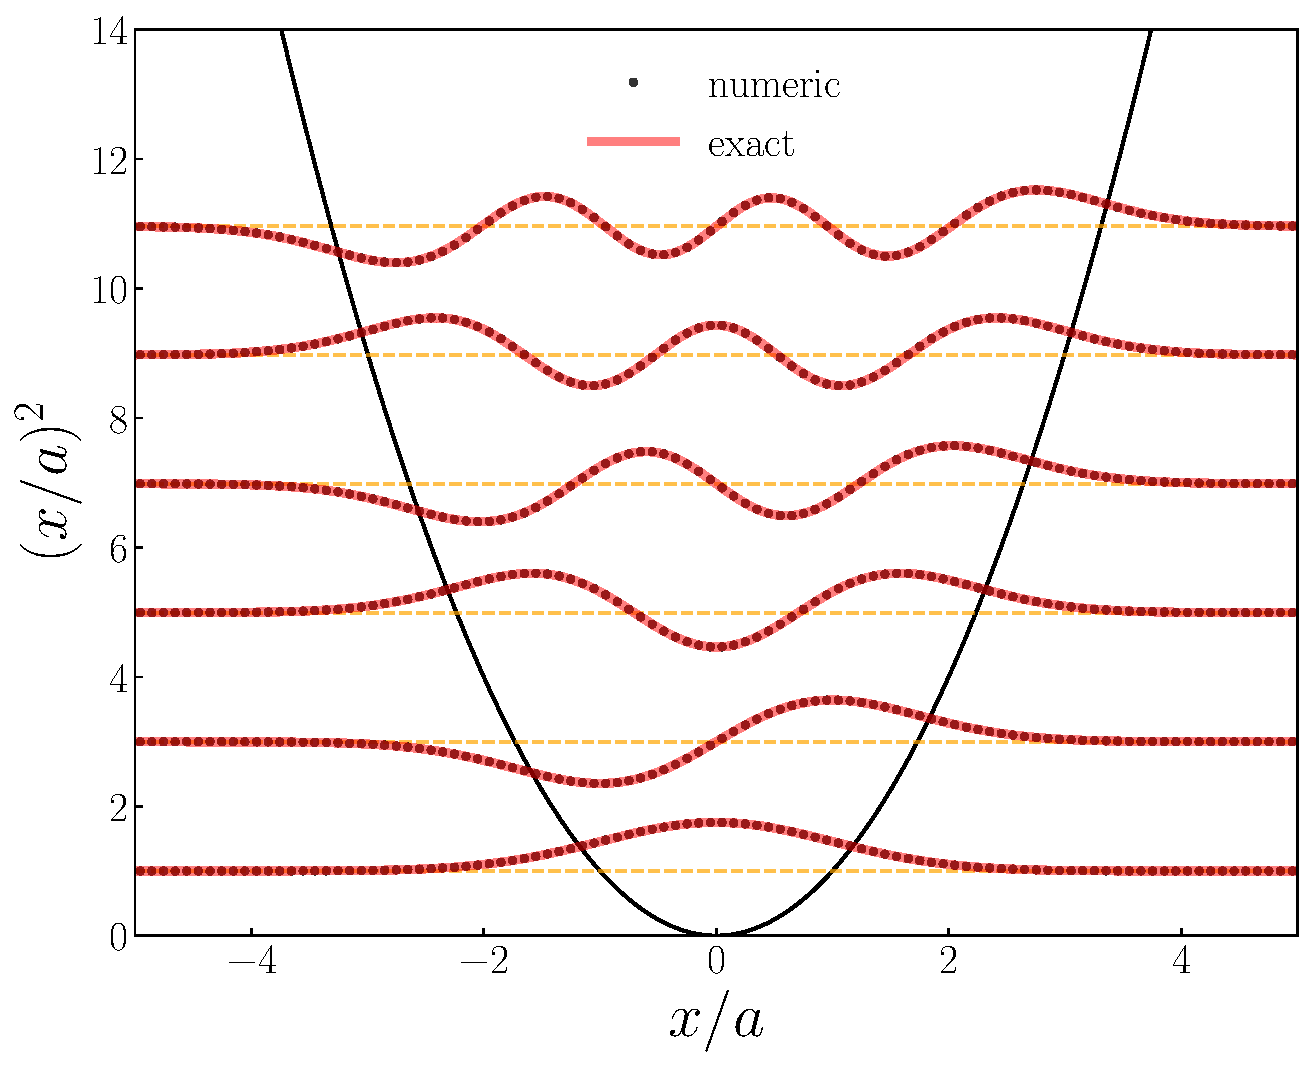
\includegraphics[width=\linewidth]{ho_wfs.pdf}
    \caption{}
    \label{fig:ho-wfs}
\end{subfigure}
\bigskip
\begin{subfigure}{0.49\linewidth}
    \centering
    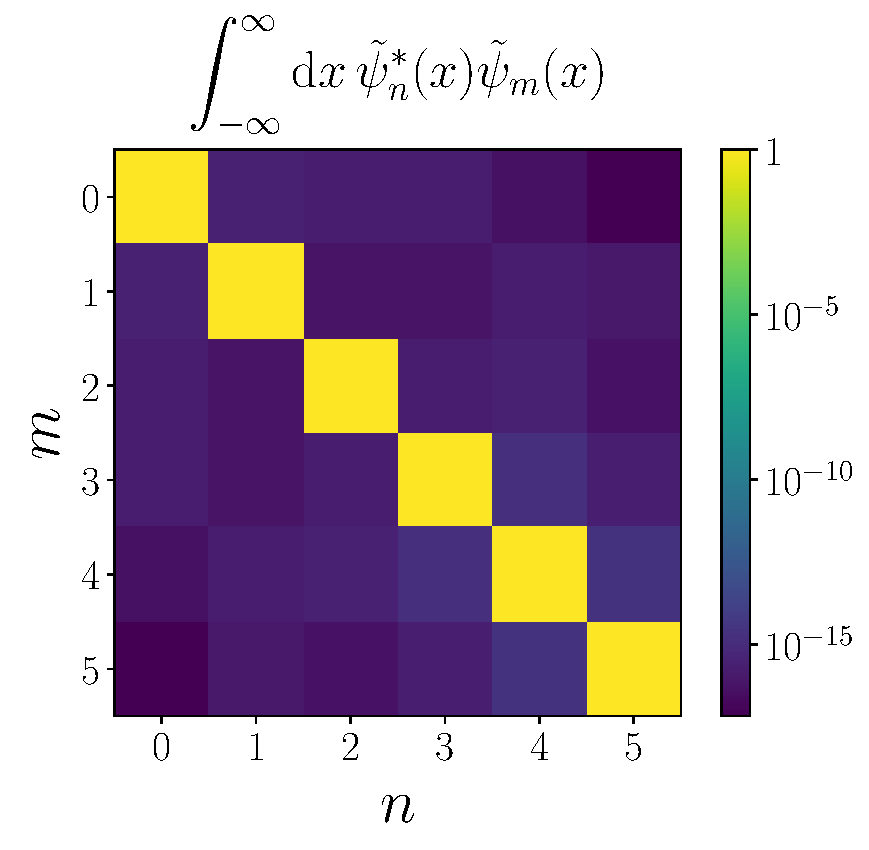
\includegraphics[width=\linewidth]{ho_orthonormality.pdf}
    \caption{}
    \label{fig:ho-orthonormality}
\end{subfigure}
\caption{\textbf{(a)} Plot of numerical and analytic results for the first six wave-functions of the quantum harmonic oscillator imposed on the potential and shifted by the energy eigenvalues. \textbf{(b)} Colormap of overlap integral between the first six wave-functions shown in (a).}
\label{fig:ho-wfs-orthonormality}
\end{figure}


\subsection{Comb potential}
\label{ssec:comb-potential}

In this section, we implement the comb well potential, which essentially repeats $N$ finite square wells of width $a$, separated by a width $b$.
For this problem, we select $a$ to be our relevant length scale and find the spectrum or energies for $N = 1,\ldots,8$ at a depth $v_0 = 50$.
The results of this exercise are shown in Fig. \ref{fig:comb-spectrum}.
A salient feature of this system is that as we increase the number of wells, we create a band structure for our spectrum, where distinct sets of bound states group together and there exists a sizable energy difference between the groups.


\begin{figure}[h!tb]
    \centering
    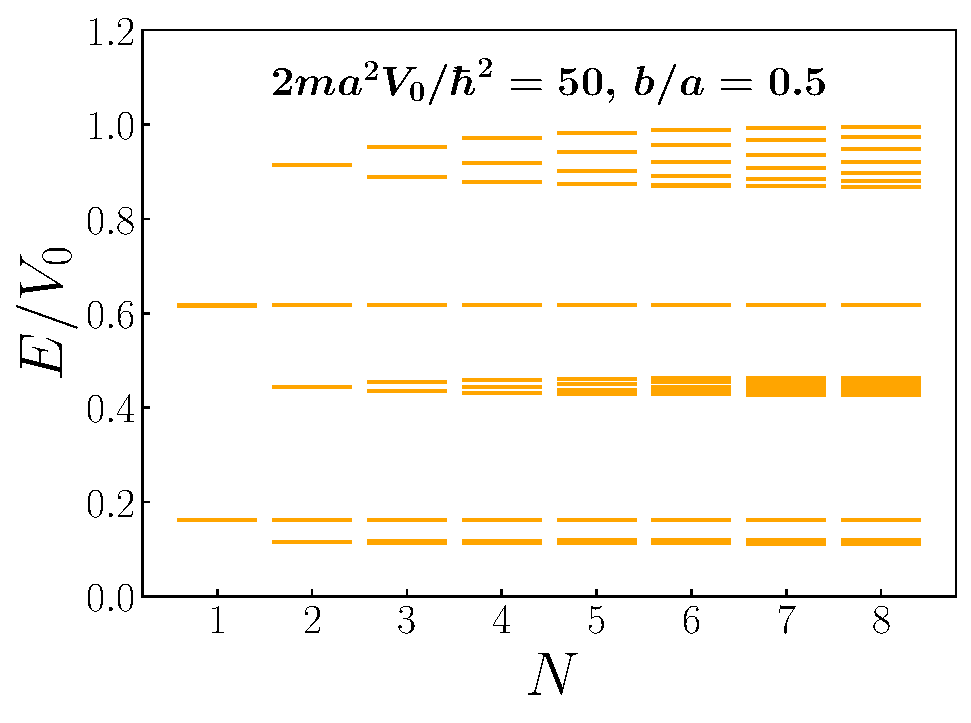
\includegraphics[width=0.5\linewidth]{comb_spectrum.pdf}
    \caption{Bound state energies for a potential made of a series of $N$ wells with width $a$ and depth $V_0 = 50 (\hbar^2 / 2 m a^2)$ separated by a width $b = a/2$.}
    \label{fig:comb-spectrum}
\end{figure}



\subsection{Morse potential}
\label{ssec:morse-potential}

Another potential we looked at was the Morse potential
\begin{align}
    V(x) = D_{e} \Big( 1 - e^{-a(x - x_0)} \Big)^2
\end{align}
which is a model used for molecules, where $D_{e}$ is the bond dissociation energy, $a$ is related to the well depth, and $x_0$ is the equilibrium separation.
In Fig. \ref{fig:morse-wfs}, we show the bound states for $2 m x_0^2 D_{e} / \hbar^2 = 20$ and $a x_0 = 0.75$.

\begin{figure}[h!tb]
    \centering
    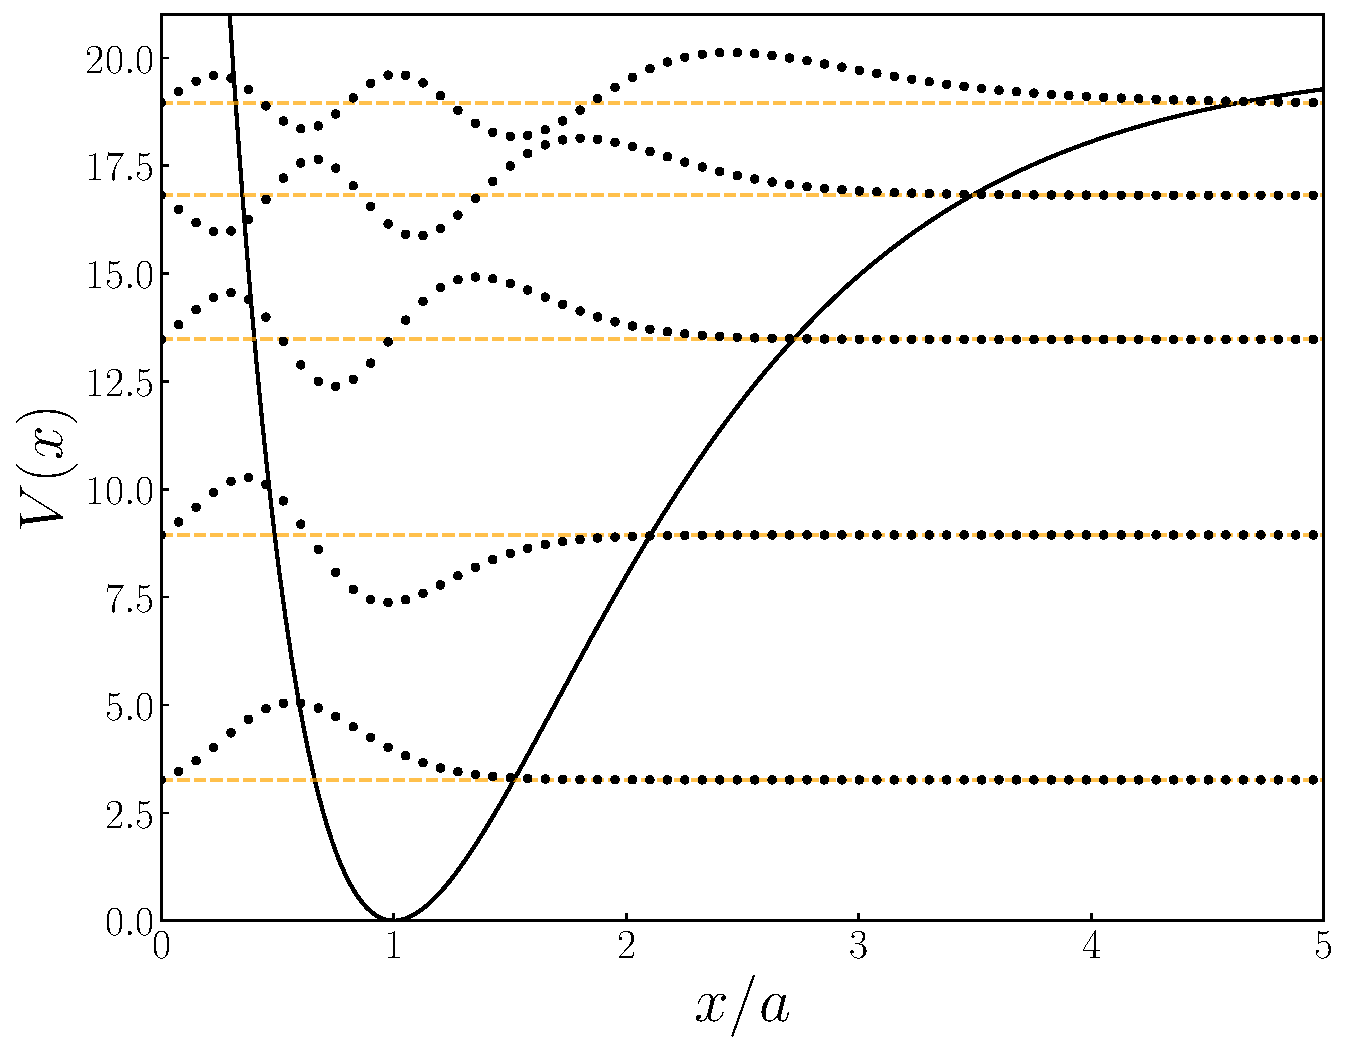
\includegraphics[width=0.5\linewidth]{morse_wfs.pdf}
    \caption{Plot of numerical results for the five wave-functions permitted by the Morse potential with $2 m x_0^2 D_{e} / \hbar^2 = 20$ and $a x_0 = 0.75$ imposed on the potential itself and offset by the bound state energies.}
    \label{fig:morse-wfs}
\end{figure}



\subsection{Hydrogen atom}
\label{ssec:hydrogen-atom}

The final potential we look at is the Coulomb potential for Hydrogen-like atoms.
In three-dimensions, for a central potential, the Schr\"{o}dinger equation reads
\begin{align}
    -\frac{\hbar^2}{2m} \grad^2 \psi(\vb*{r}) + V(r) \psi(\vb*{r}) = E \psi(\vb*{r})
.\end{align}
One can separate the angular piece of the stationary states, the spherical harmonics $Y_{\ell m}$, and the radial part $R_{n \ell}$ as $\psi_{n \ell m} = R_{n \ell}(r) Y_{\ell m}(\theta,\phi)$.
If one defines $u_{nl}(r) = R_{nl}(r) / r$, we obtain the radial equation
\begin{align}
    -\frac{\hbar^2}{2m} \dv[2]{u_{nl}(r)}{r} + \Bigg[ \frac{\hbar^2 \ell(\ell + 1)}{2m} + V(r) \Bigg] u_{n \ell}(r) = E_{n} u_{n \ell}(r)
.\end{align}
This is of the same one-dimensional form as the one we have discussed above with an effective potential
\begin{align}
    V_{\rm eff} = \frac{\hbar^2 \ell (\ell + 1)}{2 m r^2} + V(r)
\end{align}
where the first term is the so-called centrifugal barrier.
For the Coulomb potential
\begin{align}
    V(r) = -\frac{Z e^2}{r}
,\end{align}
and we can define our length-scale to be $a = a_0 / Z$, where $a_0 = \hbar^2/(m e^2)$ is the Bohr radius.
If one massages the equation using this definition, we arrive at
\begin{align}
    -\dv[2]{\tilde{u}_{n\ell}}{x} + \Bigg[ \frac{\ell (\ell + 1)}{x^2} - \frac{2}{x} \Bigg] \tilde{u}_{n \ell} = \varepsilon_{n} \tilde{u}_{n \ell}
,\end{align}
where $r = a x$.
Remarkably, this equation has an analytic solution of the form
\begin{align}
    \tilde{u}_{n \ell}(x) = \Big( \frac{2}{n} \Big)^{\ell} \sqrt{\Big( \frac{2}{n} \Big)^3 \frac{(n - \ell - 1)!}{2n (n + \ell)!}} x^{\ell + 1} e^{-x/n} L_{n-\ell-1}^{2 \ell + 1}(2x/n)
,\end{align}
where $n = 1,2,\ldots$ is the principal quantum number, $\ell = 0,\ldots,n-1$ is the angular quantum number, and $L_{q}^{p}(x)$ is an associated Laguerre polynomial.
Note that the corresponding energies $\varepsilon_{n} = -1/n^2$.
In Fig. \ref{fig:hydrogen-wfs}, we plot the first six radial wave-functions obtained numerically and analytically.
Consistent with what we have found before, the wave-functions agree to a qualitatively reasonable degree, and the energies are reproduced well.

\begin{figure}[h!tb]
    \centering
    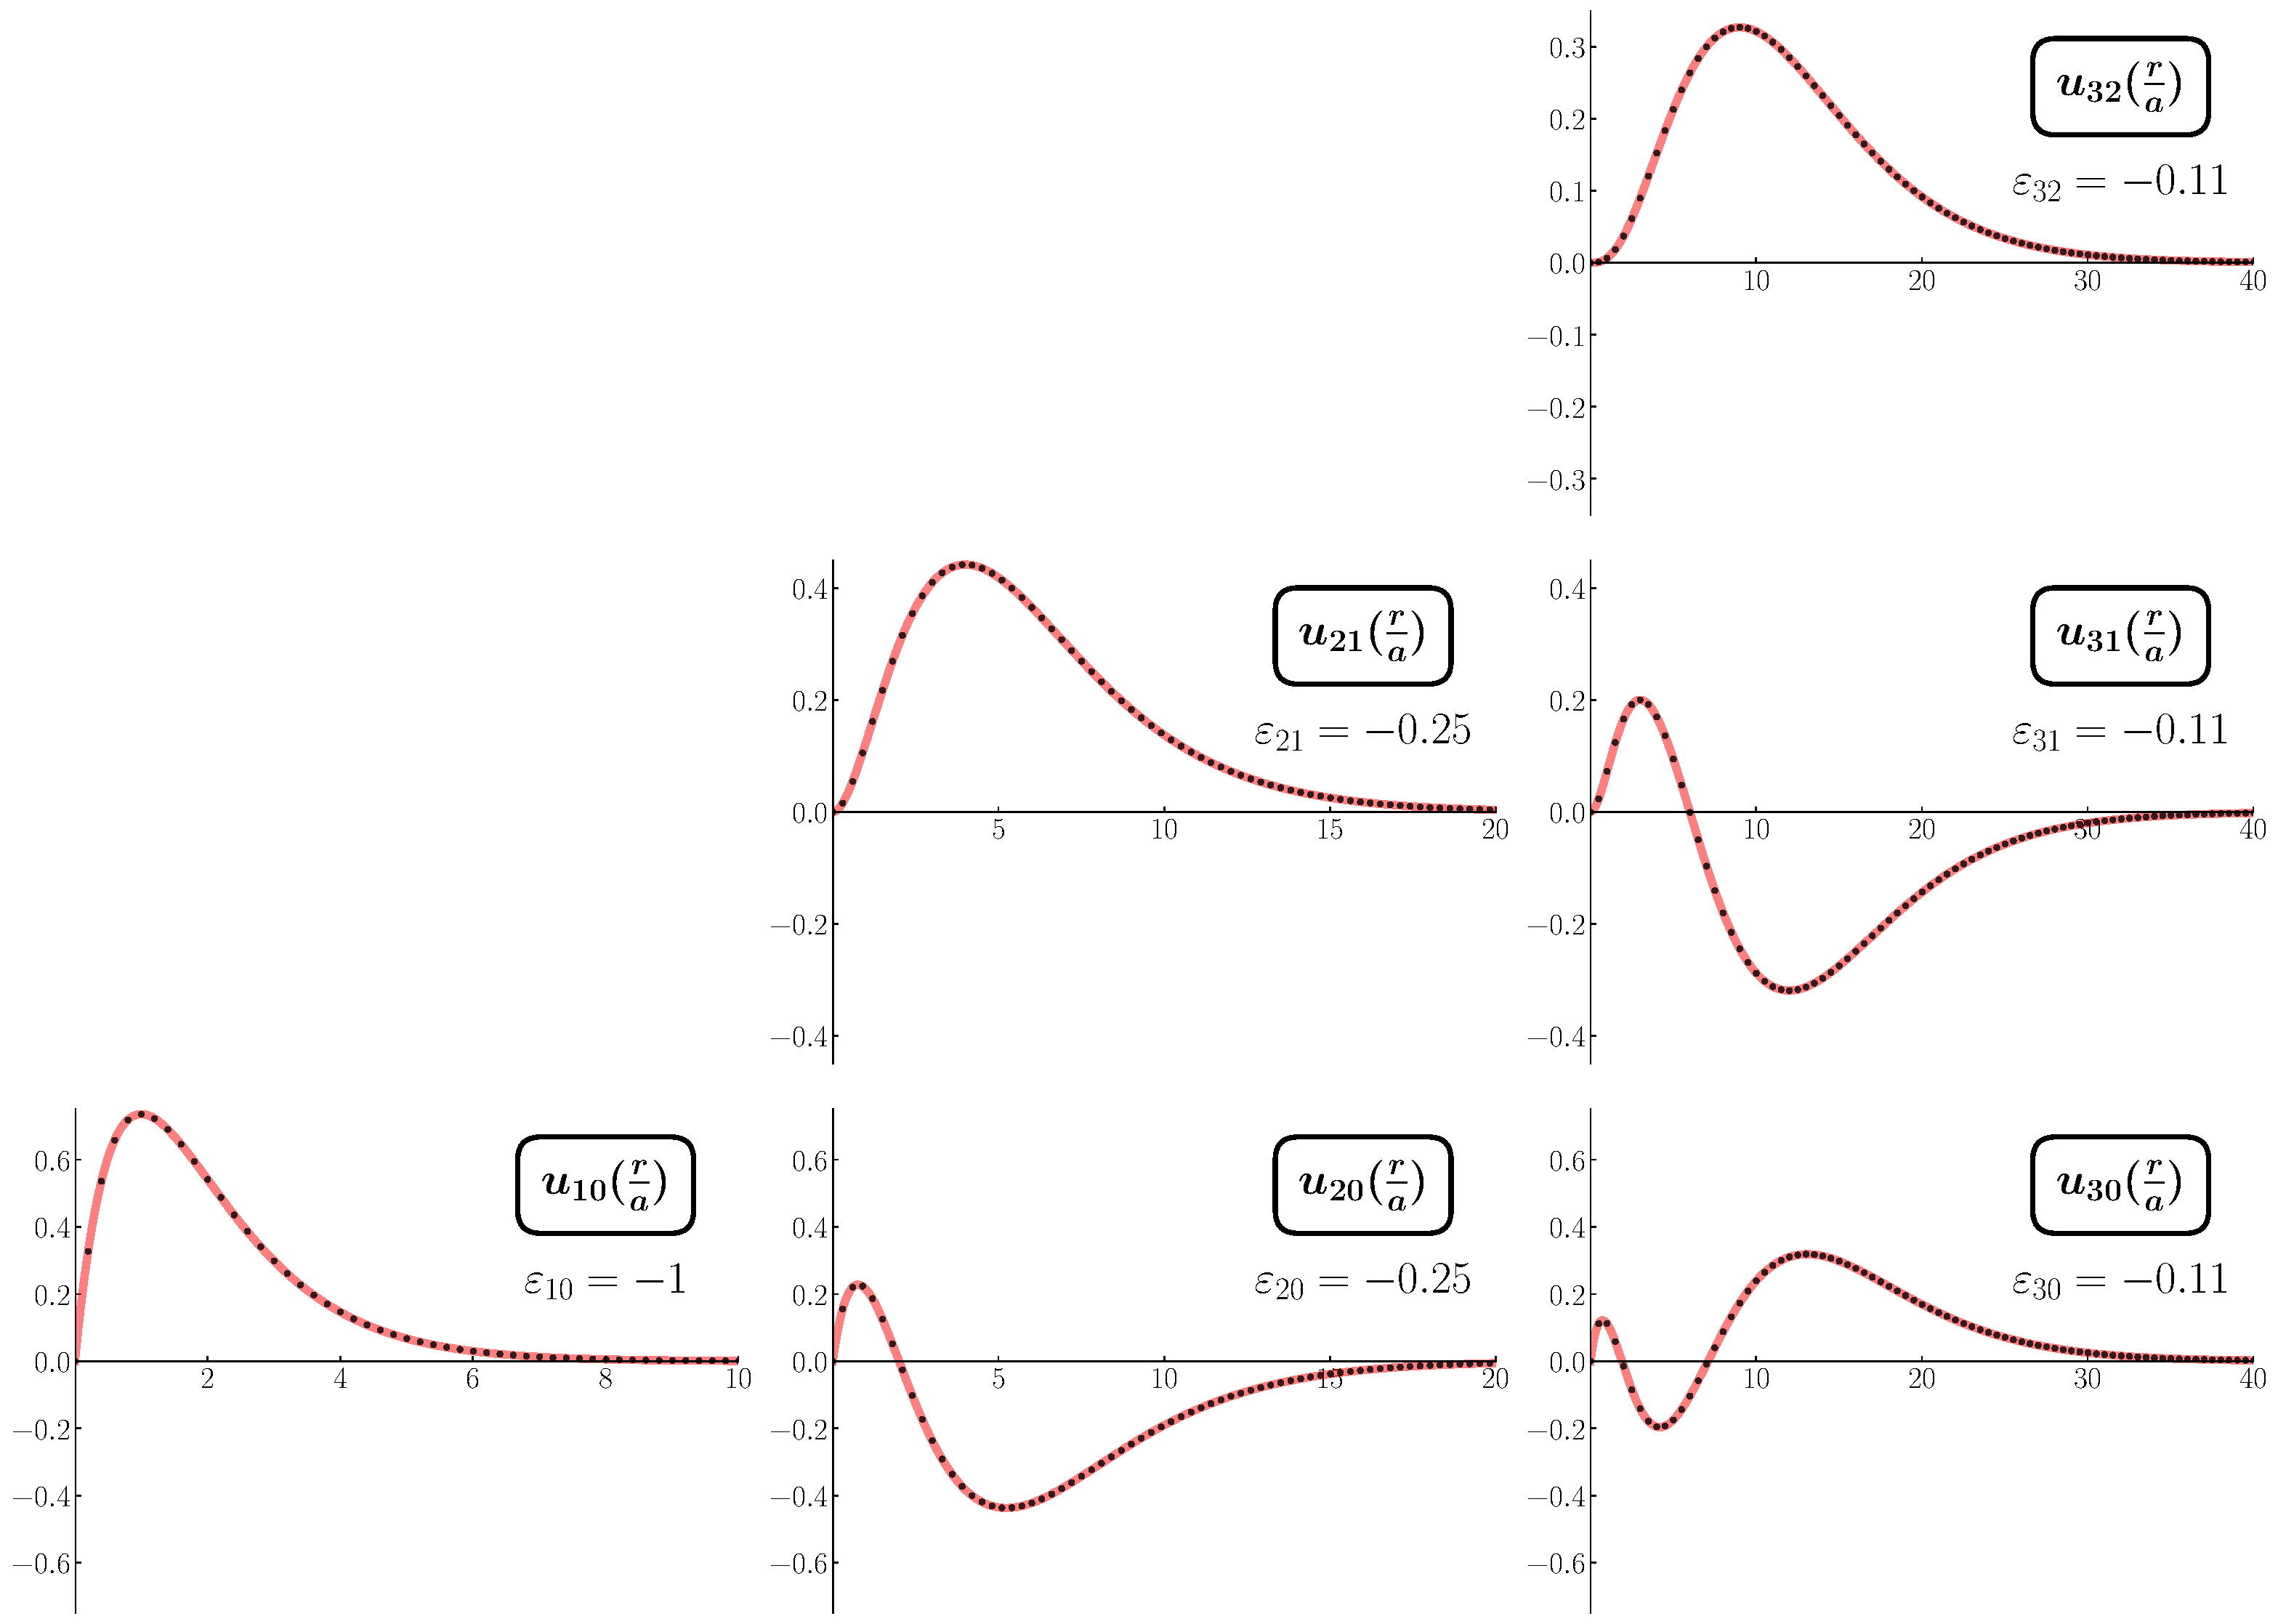
\includegraphics[width=\linewidth]{hydrogen_wfs.pdf}
    \caption{The tower of reduced radial wave-functions up to $n = 3$ for a hydrogen-like system. As usual, the solid red line denotes the analytic solution whilst the black dots denote the numerical solution.}
    \label{fig:hydrogen-wfs}
\end{figure}



\section{Conclusion}
\label{sec:conclusion}

In this work we have demonstrated a finite difference method to solve the energy eigenvalue problem for the bound states of a one-dimensional potential $V(x)$ and the corresponding bound state energies.
This method works exceptionally well for localized potentials.
During initial stages of testing, because of the sparse nature of the Hamiltonian, one could not use a large number of lattice points without encountering overflow issues in finding the spectrum of our system.
Of course, one could simply ask for only a limited number of eigenstates and eigenvalues, but because of the construction of the second-derivative in the finite difference method, our Hamiltonian matrix becomes tridiagonal on the lattice, allowing us to leverage numerical methods designed to efficiently determine the eigenvectors and eigenvalues of such matrices.
This enabled us to achieve a high accuracy by enlarging the interval of consideration and increasing the lattice density to a very high level.

In research settings, solving problems on a lattice can be quite memory intensive.
While this method can be extended to two or three dimensions, in order to achieve a high enough lattice density to sufficiently suppress the error terms of our finite difference methods, we must scale the number of lattice points exponentially.
Additionally, while many one-body or two-body systems can be modeled as in the section addressing the hydrogen atom, we cannot do so with a three-body or larger system.
To address these issues one could implement these programs on a high performance computing system.
Alternatively, either a more accurate finite difference formula could be used, although this would induce more off-diagonal matrix elements in our Hamiltonian and require a different eigensolver, or another solution method should be implemented, perhaps based on a monte carlo methodology.
Whatever the approach, though, it is vital that we be able to solve the Schr\"{o}dinger equation given its importance in understanding fundamental, small-scale systems in nature.

    
\end{document}
